\section{Руководство по использованию}
\quad {Для начала работы необходимо запустить программу}.
Для этого не обходимо нажать два раза по иконке приложения или выделить и уже после этого нажать клавишу enter.\\
\quad {После} запуска в консоли появится сообщение о необходимости нажатия кнопок 1 и 2 для перевода геймпада в режим синхронизации.
Также есть альтернатива в виде нажатия отельной кнопки синхронизации в отсеке с аккумуляторами.
После чего должна пройти синхронизация.
В случае успешного установления синхронизации будет выведено сообщение, оповещающее пользователя об этом.
\quad Совместно с этим сообщением будет выведена инструкция о работе с геймпадом.\\
\quad Инструкция:\\
\begin{itemize}
    \item Нажимайте кнопки 1 или 2 для изменения состояния светодиодного индикатора.
    \item Нажмите B для включения/отключения вибрации.
    \item Нажмите A, чтобы включить/отключить акселерометр.
    \item {Одновременно нажмите A и Минус, чтобы отключить геймпад.}
\end{itemize}
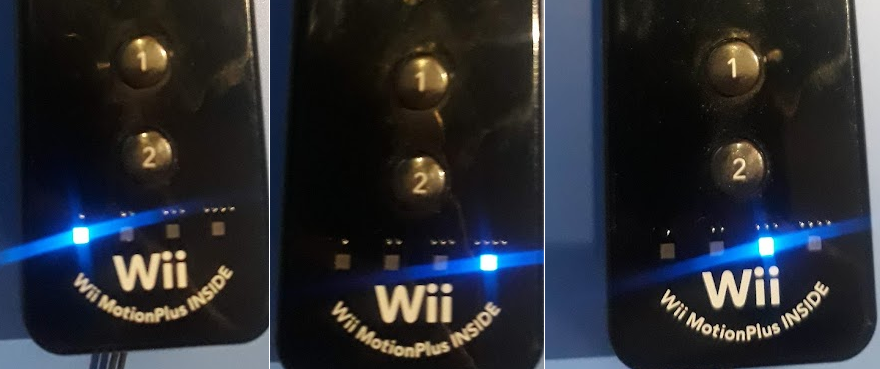
\includegraphics[width=\textwidth]{content/LedsChange}
\captionof{figure}{Пример переключения светодиодов с помощью клавиш 1 и 2}
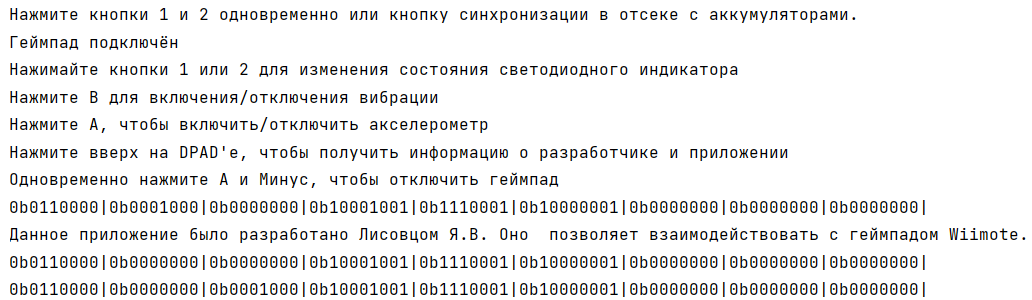
\includegraphics[width=\textwidth]{content/ProgramOutput}
\captionof{figure}{Пример работы программы}